\documentclass[12pt, a4paper]{report}
\usepackage[utf8]{inputenc}
\usepackage{hyperref} 
\usepackage{graphicx}
\graphicspath{ {./images/} }
\title{Machine Learning Course Project}

\begin{document}
    %\maketitle
    %\tableofcontents
    \section{Problem formulation}
    \subsection{Application of ML Problem}
    The current winter has shown that slippery weather might come as a surprise.
    However, when slippery conditions are expected during the day, a service called \href{https://liukastumisvaroitus.fi/en/}{Liukastumisvaroitus (link)} (Slipping warning) sends subscribers a text-message.

    According to the website, the slippery condition is identified by humans.
    Though one could think that these dangerous weather conditions can be predicted without 
    human knowledge, but to what level of accuracy? This makes it a great target for testing machine learning as an application.
    
    Ideally the machine learning application could predict, given the current weather conditions, whether the slippery warning would be raised.

    The data point is going to be a daily observation of weather data, with the additional
    slippery warning parameter. In other words, a single data point represents the weather conditions of a day. Data includes all data points (daily observations) from around 
    October 2011, as the earliest records of slipping warnings are from then.

    Concluding the parameters, 
    \begin{itemize}
      \item Potential features for the application could be \textit{Precipitation amount}, \textit{Air temperature} and \textit{Snow depth}. All of these properties are numerical and are easily measureable.
      \item The label of the application is going to be whether the \textit{slippery warning} would be raised, with values 0/1.
    \end{itemize}
    
    \section{Methods}

    \subsection{Data sources}
    The slipping warning service offers an API \cite{warnsource} for historical data analysis. Some 600 warnings have been issued in total since October 2011.
    %The slipping warning can be seen to be given at any point during the day, though most usually in the night hours.
    Additionally, the slipping warnings are given on city level for Lahti, Oulu, Kuopio, Jyväskylä, Helsinki, and Joensuu.
    As the slipping warning service data only consists of a timestamp and the city issued, training the machine learning algorithm to account for the current weather conditions needs more data to work with.

    Thus, historical weather data from the Finnish Metheorological Institute \cite{fmisource}
    is combined. Although FMI offers hourly historical data, in this project, the plan is to use the daily aggregated weather recordings for simplicity.
    In total, there are some 3800 (days) * 6 (cities) $\approx$ 23000 daily weather reports since October 2011.
    The FMI data includes air temperature (min/max/overall), ground temperature, precipitation amount and snow depth, which can be used as features in this project.

    Combined together based on the city and the date value, these data sources will be used to train and validate the machine learning algorithm. 
    The labels and features are extracted from the sources and used as explained in the \hyperlink{section.0.1.1}{introduction section}. 
    In total we get some 23000 data points for the ML application.

    \subsection{Feature selection}
    When you think what causes the most dangerous slipping conditions outside, two conditions need to apply:
    \begin{itemize}
      \item There need to be ice on the road.
      \item There need to be water on the road.
    \end{itemize}
    These conditions are the result of a weather that's around 0°C in temperature and the environment is snowy or there's waterfall happening.
    Thus, features selected are \textbf{Air temperature}, \textbf{Maximum temperature}, \textbf{Precipitation amount} and \textbf{Snow depth}. Empirical feature analysis 
    and comparison using my ML script and Excel back up these selections. 

    Feature candidates, such as Ground level minimum temperature, was cut off due to lack of data.
    As slipping conditions occur more often when there's snow to be melted away than when ice is forming, maximum temperature can
    suggest better than minimum temperature. Minimum temperature was then left out from the features after analysis.

    \subsection{Model}
    The model selected is the k nearest neighbor algorithm. By \autoref{fig:knnfig}, the algorithm looks at closest k data points
    to the classification target point and determines the class based on which classes have advantage of prevalence in the area.
    \begin{figure}
      \caption{Example of a nearest neighbor classification problem. Cite: \cite{knnimage}}\label{fig:knnfig}
      \centering
      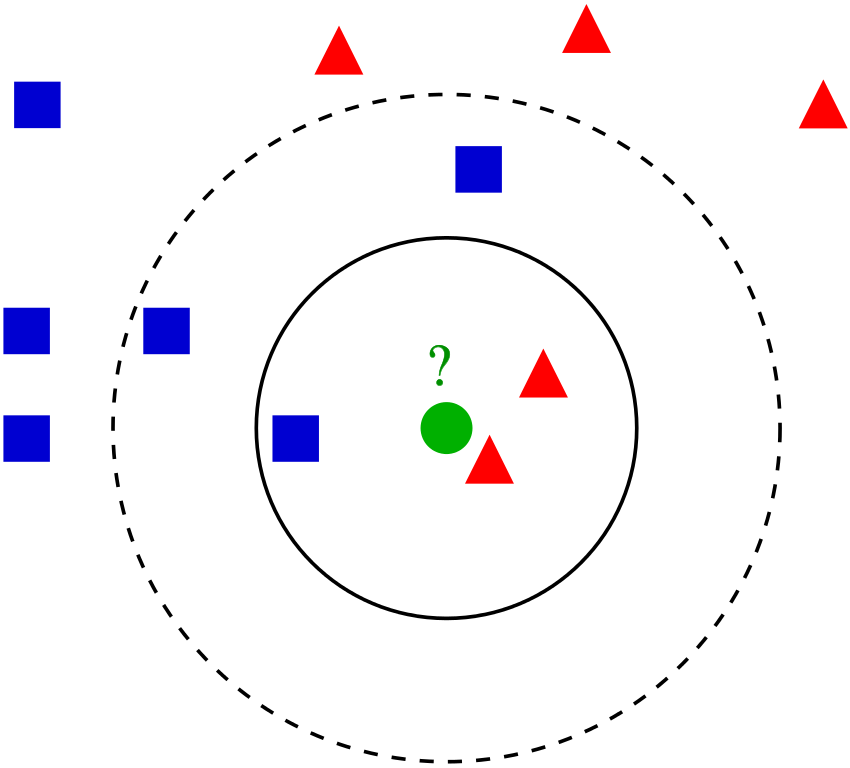
\includegraphics[width=0.4\columnwidth]{KnnClassification.svg.png}
    \end{figure}

    As the ML problem is clearly a classification type, I chose a classification method.
    Analysing different classification models led to chosing this model, as the accuracy was the greatest. 
    Since there seems to be slim boundaries in the weather metrics when issuing a slipping warning or not, the nearest neighbor
    algorithm can identify even the smallest variations and hopefully lead to good results.

    \subsubsection{Loss function}
    By course material, 0/1 loss is considered the default loss function for especially the k-nearest neighbors classification model. Thus, it is a 
    good starting point for evaluating the model performance and it is chosed as the loss function in this phase. It gives a 
    simple enough performance figure, essentially measuring the accuracy of classification (function \textit{accuracy\_score} from sklearn).
    \subsection{Data set construction}
    As the amount of slipping warnings is quite low compared to the actual weather observations (600 $<$ 23000), performng a random split once might lead to 
    very polarised results regarding the contained warnings. Thus, k-fold approach is used to mitigate the random split variations better.

    Training and validation data is splitted with the k-fold approach. K-fold runs the training and validation cycle multiple times for different
    subsets of the data. Data consists of some 23000 data points, which is splitted in to 5 folds as it is the default in the sklearn utility. 
    Folding 5 times results in a training set of 18000 data points and a validation set of 5000 data points in each run.
    
    %\newpage

    \section{Appendices}
    \begin{itemize}
      \item Code and resources are available on the github page: \href{https://github.com/aksun1/cs-c3240-ml-project}{Link}.
    \end{itemize}

    \newpage

    \begin{thebibliography}{9}
      \bibitem{warnsource}
      Slipping warning service API, \href{https://liukastumisvaroitus-api.beze.io/api/v1/warnings/}{https://liukastumisvaroitus-api.beze.io/api/v1/warnings/}
      \bibitem{fmisource}
      Finnish Metheorological Institute, observation history \href{https://en.ilmatieteenlaitos.fi/download-observations}{https://en.ilmatieteenlaitos.fi/download-observations}
      \bibitem{knnimage}
      Antti Ajanki AnAj, CC BY-SA 3.0 \href{http://creativecommons.org/licenses/by-sa/3.0/}{http://creativecommons.org/licenses/by-sa/3.0/}, via Wikimedia Commons (\href{https://commons.wikimedia.org/wiki/File:KnnClassification.svg}{https://commons.wikimedia.org/wiki/File:KnnClassification.svg})
    \end{thebibliography}


\end{document}